\chapter{Implementación del sistema de vuelo con ROS}

En esta última sección de resultados se desglosa el proceso llevado a cabo para la implementación de los nodos del algoritmo de visión artificial y el seguimiento de trayectoria. Cabe mencionar que en esta última parte no es tan extensa como las anteriores, pues básicamente la creación de los nodos puede ser vista como un proceso de integración. De hecho, se parte de lo últimos códigos desarrollados en cada sección, de tal forma que el contenido de cada nodo es en esencia lo desarrollado en su respectiva subsección.

\section{Visión Artificial}
La implementación del algoritmo de detección de compuertas fue quizás la más sencilla, pues al utilizar funciones básicas de OpenCV, no fue necesario incluir librerías adicionales, quizás el cambio más representativo con respecto al programa mencionado en la sección del sistema de visión artificial es la inclusión de la librería \textit{cv\_bridge.h}, la cual permite realizar la conversión entre una imagen recibida por un topic de ROS a un formato que OpenCV sea capaz de manejar. Entonces, la implementación de la aplicación resultó ser bastante intuitiva y práctica.

A partir de lo anterior, el paradigma para la conversión entre un programa de programación estructura a un nodo de ROS es sencillo en mucho de los casos, pues la consideración más importante que se tiene que realizar es que, al ser un nodo de ROS, el programa se estará ejecutando como un proceso dentro del sistema operativo, de tal manera que su ejecución se hará de forma indefinida a manera de ciclo. Entonces, el algoritmo \ref{alg:ROS_vision} ejemplifica a grandes rasgos la lógica implementada. Se puede observar que la secuencia a seguir es sencilla; sin embargo, quizás lo que puede llegar a consumir más tiempo al realizar este tipo de porteo son las consideraciones que se tiene que realizar dentro de la programación orientada a objetos (POO), que si bien un nodo de ROS puede ser implementado con lógica secuencial, el uso de POO simplifica bastante la cantidad de código.


\begin{algorithm}
    \caption{Nodo de visión artificial para la detección de compuertas}\label{alg:ROS_vision}
    \begin{algorithmic}
    \While{True}
    \State \textbf{Leer} topic de transmisión de imagen de cámara
    \State \textbf{Convertir} tipo de imagen de ROS a OpenCV
    \State \textbf{Ejecutar} algoritmo de visión artificial
    \EndWhile
\end{algorithmic}
\end{algorithm}

Ahora, las figuras \ref{fig:ROS_gate1}, \ref{fig:ROS_gate2}, \ref{fig:ROS_gate3}, \ref{fig:ROS_gate4} presentan el desempeño del algoritmo dentro de la simulación, en donde cada conjunto de imágenes corresponde al momento en que la cámara del dron tiene en su campo de visión a cada una de las compuertas que componen el circuito de vuelo. Hablando de manera general, cada grupo de imágenes contiene un total de 8 sub-imágenes, en donde la primera fila de imágenes muestra el fotograma original captado por la cámara del dron, y la segunda fila contiene el respectivo resultado asociado al procesamiento de cada uno de estos fotogramas.

Hablando de forma más detallada sobre cada conjunto de imágenes, la figura \ref{fig:ROS_gate1} presenta la secuencia de acercamiento que el dron realizó con respecto a la primera compuerta. Es posible resaltar el hecho de que, a pesar de tener un edifico con una fachada roja, el algoritmo fue capaz de aislar la compuerta con éxito; la detección se hace de forma gradual y mejora conforme el dron acorta la distancia con la compuerta.

\begin{figure}[ht]
    \centering
    \subfloat[ ]{\label{fig:ROS_gate1og1}{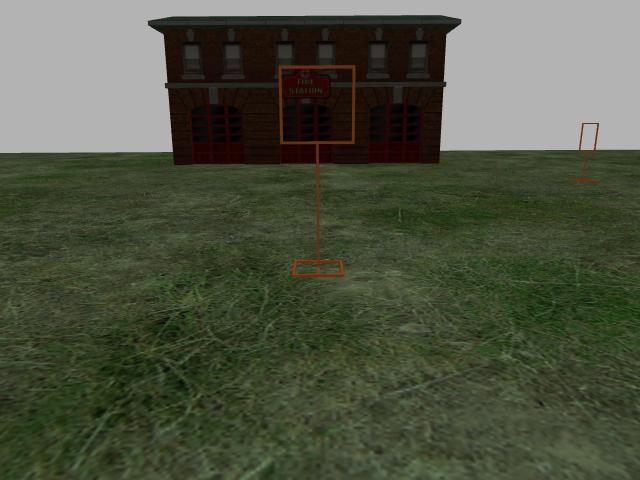
\includegraphics[width=0.2\textwidth]{ROS_gate1og1.png}}} \hspace{0.2 pt}
    \subfloat[ ]{\label{fig:ROS_gate1og2}{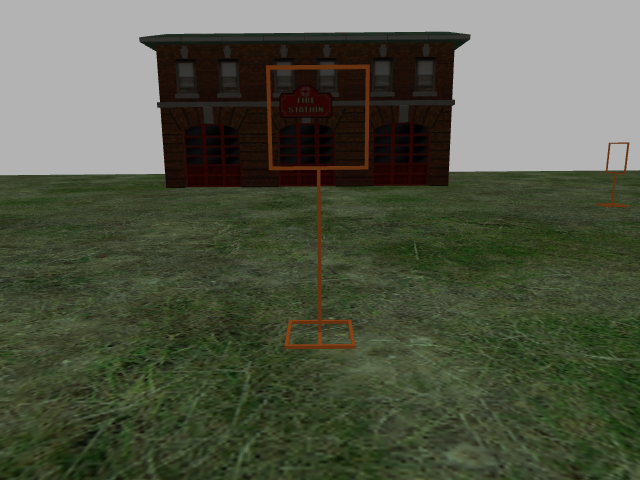
\includegraphics[width=0.2\textwidth]{ROS_gate1og2.png}}} \hspace{0.2 pt}
    \subfloat[ ]{\label{fig:ROS_gate1og3}{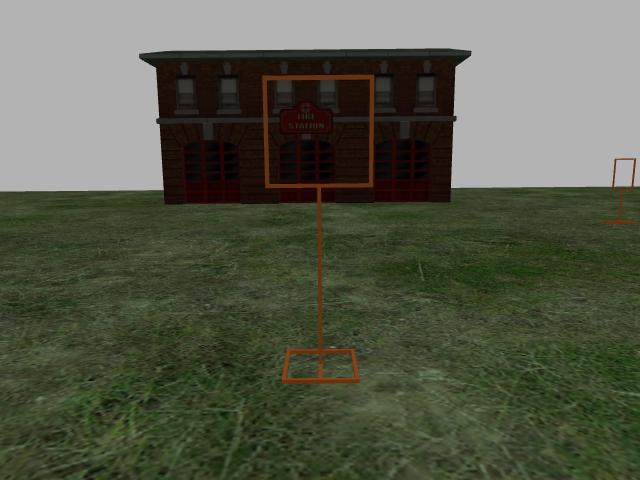
\includegraphics[width=0.2\textwidth]{ROS_gate1og3.png}}} \hspace{0.2 pt}
    \subfloat[ ]{\label{fig:ROS_gate1og4}{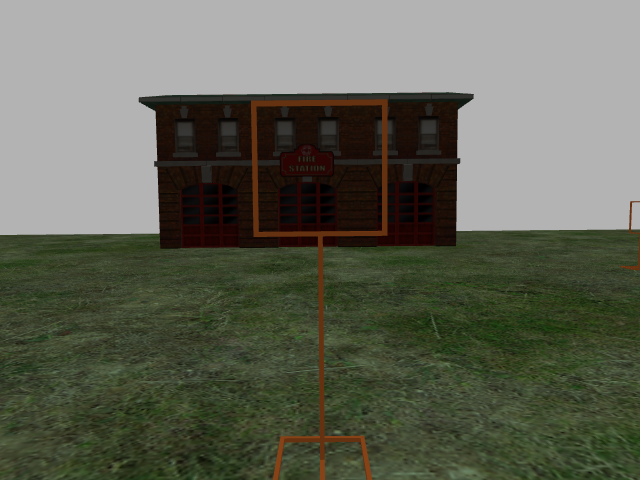
\includegraphics[width=0.2\textwidth]{ROS_gate1og4.png}}} \\
    \subfloat[ ]{\label{fig:ROS_gate1th1}{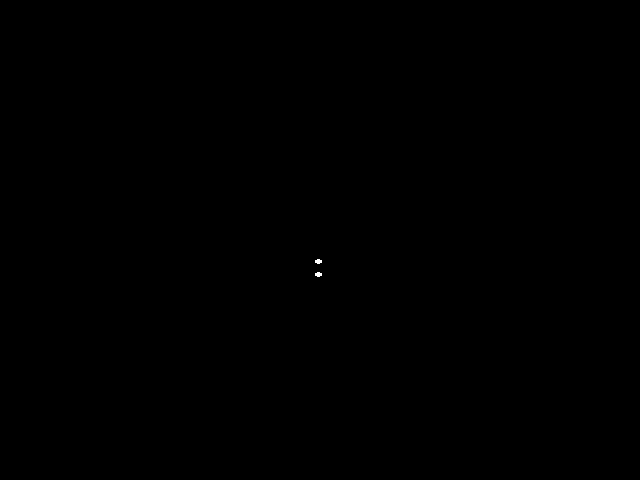
\includegraphics[width=0.2\textwidth]{ROS_gate1th1.png}}} \hspace{0.2 pt}
    \subfloat[ ]{\label{fig:ROS_gate1th2}{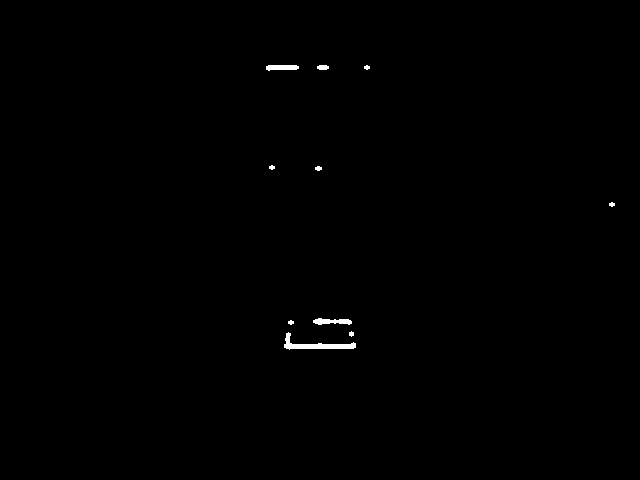
\includegraphics[width=0.2\textwidth]{ROS_gate1th2.png}}} \hspace{0.2 pt}
    \subfloat[ ]{\label{fig:ROS_gate1th3}{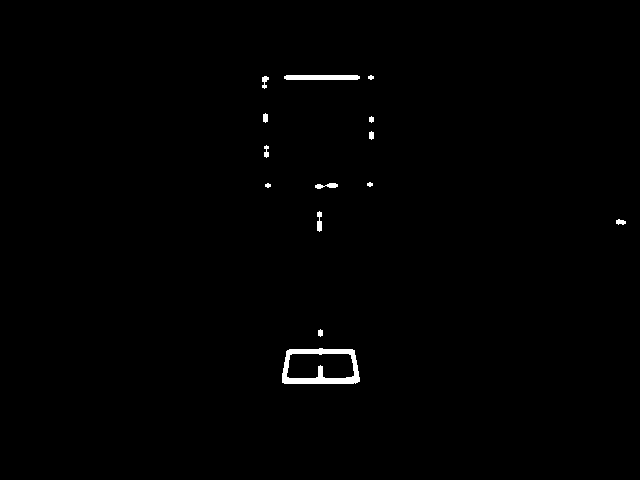
\includegraphics[width=0.2\textwidth]{ROS_gate1th3.png}}} \hspace{0.2 pt}
    \subfloat[ ]{\label{fig:ROS_gate1th4}{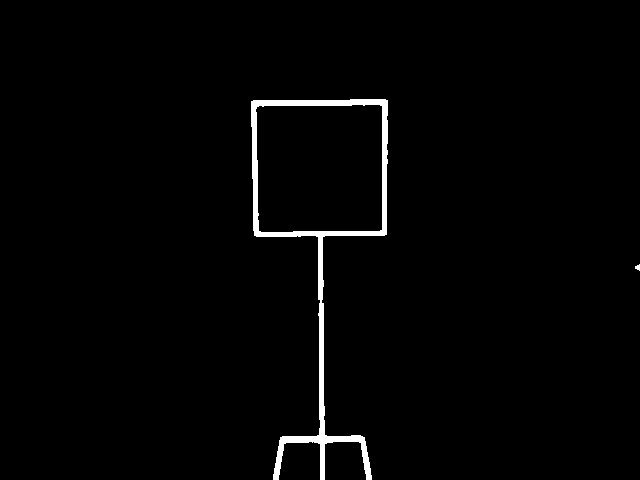
\includegraphics[width=0.2\textwidth]{ROS_gate1th4.png}}}
    
    \caption{Detección de la primera compuerta}
    \label{fig:ROS_gate1}
\end{figure}

Después, la figura \ref{fig:ROS_gate2} contiene la secuencia de fotogramas asociada a la detección de la segunda compuerta, en este caso en particular no existe otro objeto de gran tamaño que puede afectar la detección de forma significativa; sin embargo, es importante mencionar que esta compuerta en específico es de una altura menor en comparación con el resto de compuertas, además, también es posible hacer hincapié en que en algunos de los fotogramas se observa las palas de algunos de los motores del dron. En este caso la detección fue más limpia en comparación al anterior.

\begin{figure}[ht]
    \centering
    \subfloat[ ]{\label{fig:ROS_gate2og1}{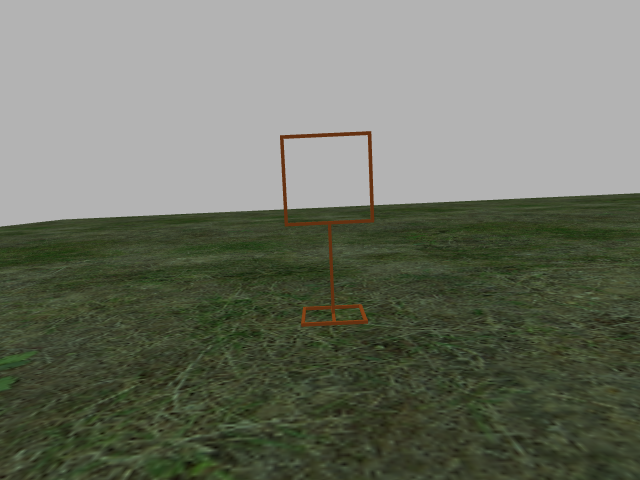
\includegraphics[width=0.2\textwidth]{ROS_gate2og1.png}}} \hspace{0.2 pt}
    \subfloat[ ]{\label{fig:ROS_gate2og2}{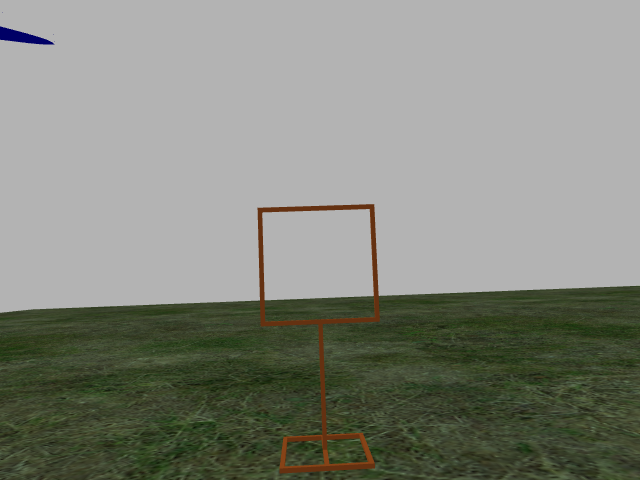
\includegraphics[width=0.2\textwidth]{ROS_gate2og2.png}}} \hspace{0.2 pt}
    \subfloat[ ]{\label{fig:ROS_gate2og3}{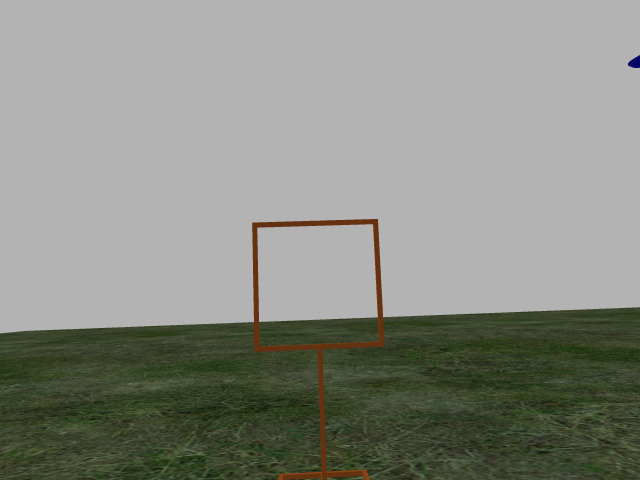
\includegraphics[width=0.2\textwidth]{ROS_gate2og3.png}}} \hspace{0.2 pt}
    \subfloat[ ]{\label{fig:ROS_gate2og4}{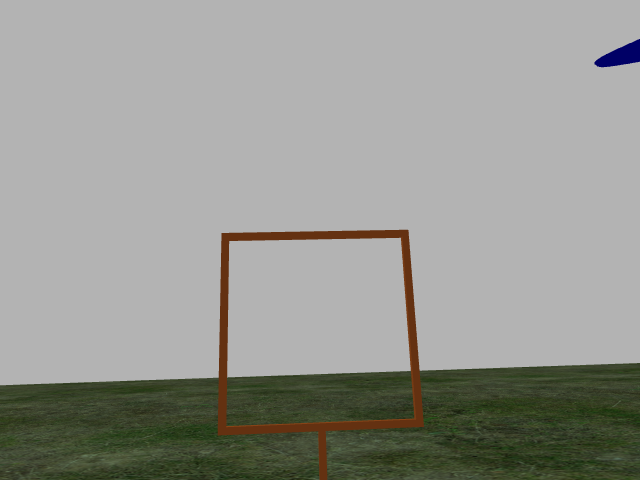
\includegraphics[width=0.2\textwidth]{ROS_gate2og4.png}}} \\
    \subfloat[ ]{\label{fig:ROS_gate2th1}{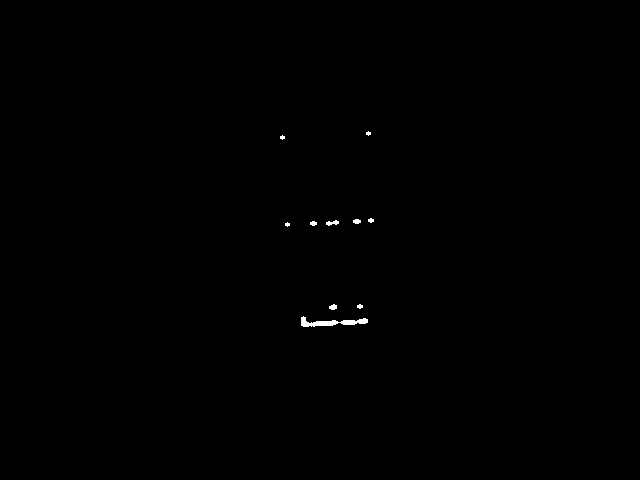
\includegraphics[width=0.2\textwidth]{ROS_gate2th1.png}}} \hspace{0.2 pt}
    \subfloat[ ]{\label{fig:ROS_gate2th2}{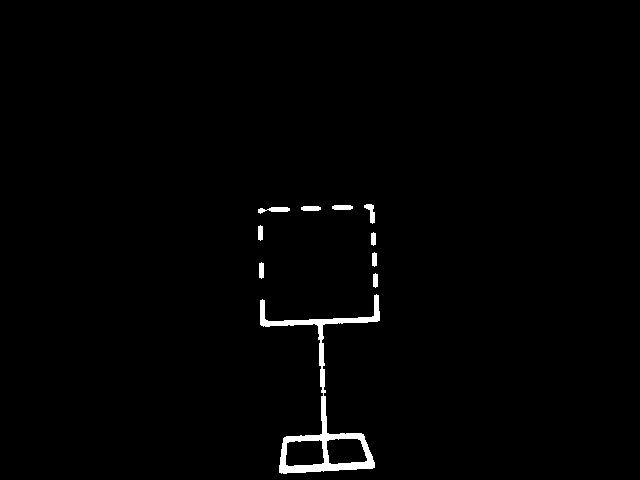
\includegraphics[width=0.2\textwidth]{ROS_gate2th2.png}}} \hspace{0.2 pt}
    \subfloat[ ]{\label{fig:ROS_gate2th3}{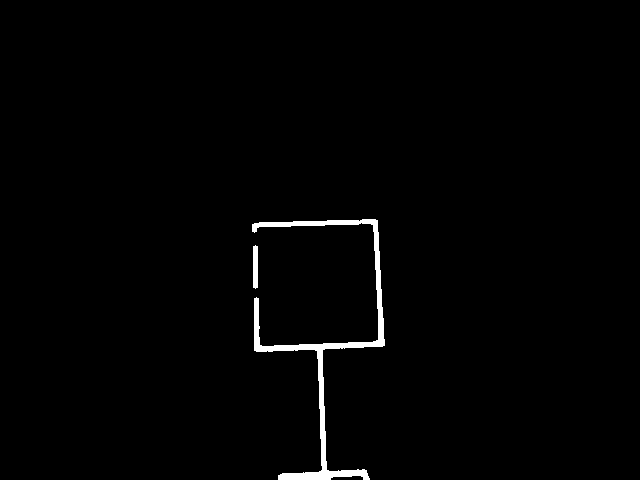
\includegraphics[width=0.2\textwidth]{ROS_gate2th3.png}}} \hspace{0.2 pt}
    \subfloat[ ]{\label{fig:ROS_gate2th4}{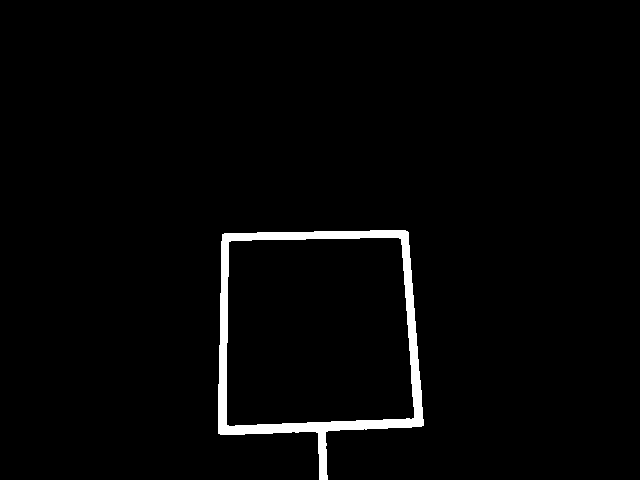
\includegraphics[width=0.2\textwidth]{ROS_gate2th4.png}}}
    
    \caption{Detección de la segunda compuerta}
    \label{fig:ROS_gate2}
\end{figure}


Continuando con el análisis, la figura \ref{fig:ROS_gate3} presenta el desempeño obtenido para la detección de la tercera compuerta. En este caso es posible apreciar de mejor manera el efecto que tiene la distancia con respecto al objeto de interés al momento de realizar la detección. Se observa que, a pesar de que no existe una gran cantidad de objetos que puedan afectar el funcionamiento del algoritmo, este no es capaz de detectar las compuertas a grandes distancias, a pesar de que se encuentren dentro de su campo de visión, es más, en este caso se aprecia que no se detectó la compuerta completa, pues cuando el algoritmo fue capaz aislar por completo el objeto, el dron ya se encontraba a una distancia en donde el campo de visión de la cámara no enfoca toda la compuerta.

\begin{figure}[ht]
    \centering
    \subfloat[ ]{\label{fig:ROS_gate3og1}{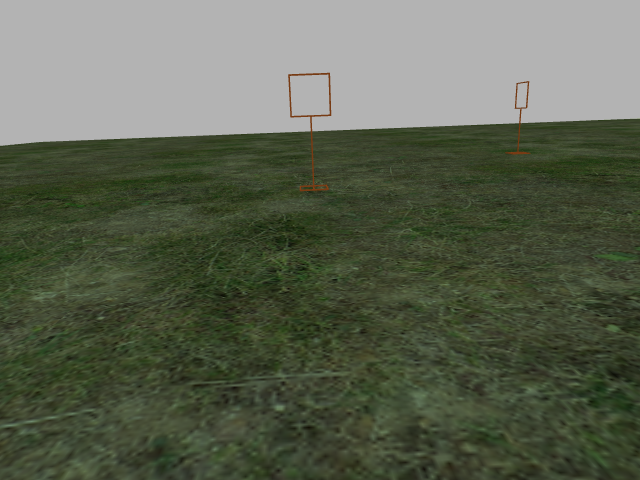
\includegraphics[width=0.2\textwidth]{ROS_gate3og1.png}}} \hspace{0.2 pt}
    \subfloat[ ]{\label{fig:ROS_gate3og2}{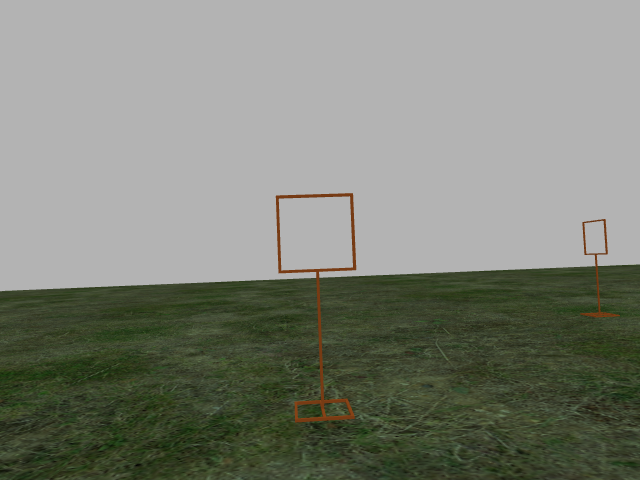
\includegraphics[width=0.2\textwidth]{ROS_gate3og2.png}}} \hspace{0.2 pt}
    \subfloat[ ]{\label{fig:ROS_gate3og3}{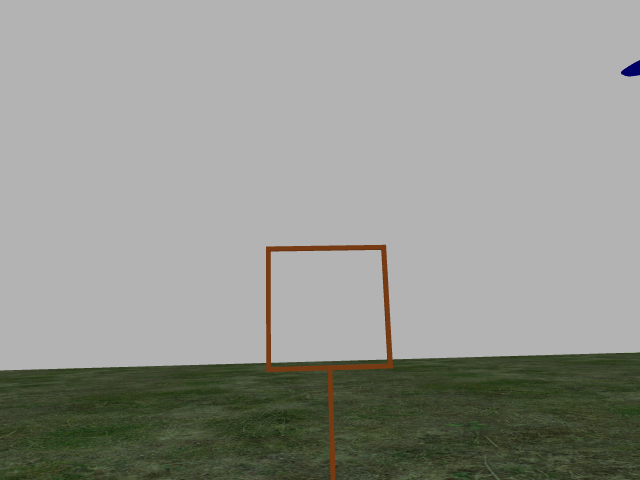
\includegraphics[width=0.2\textwidth]{ROS_gate3og3.png}}} \hspace{0.2 pt}
    \subfloat[ ]{\label{fig:ROS_gate3og4}{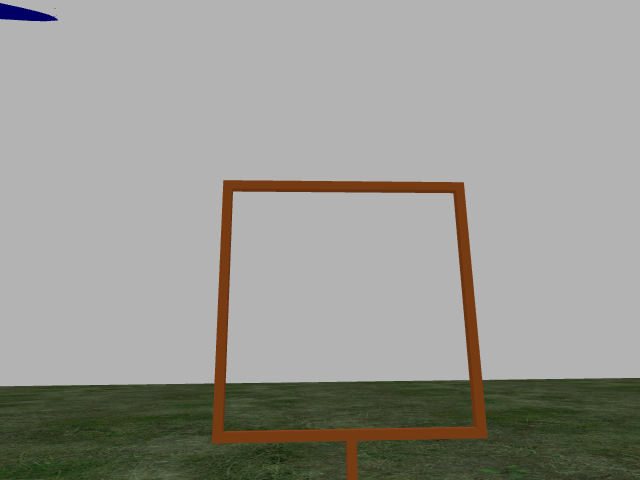
\includegraphics[width=0.2\textwidth]{ROS_gate3og4.png}}} \\
    \subfloat[ ]{\label{fig:ROS_gate3th1}{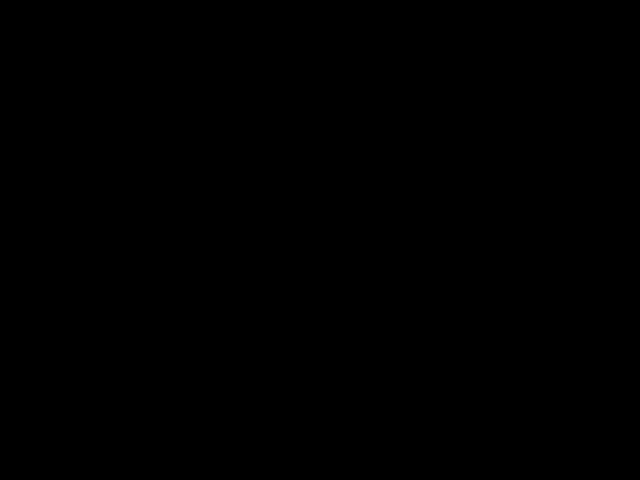
\includegraphics[width=0.2\textwidth]{ROS_gate3th1.png}}} \hspace{0.2 pt}
    \subfloat[ ]{\label{fig:ROS_gate3th2}{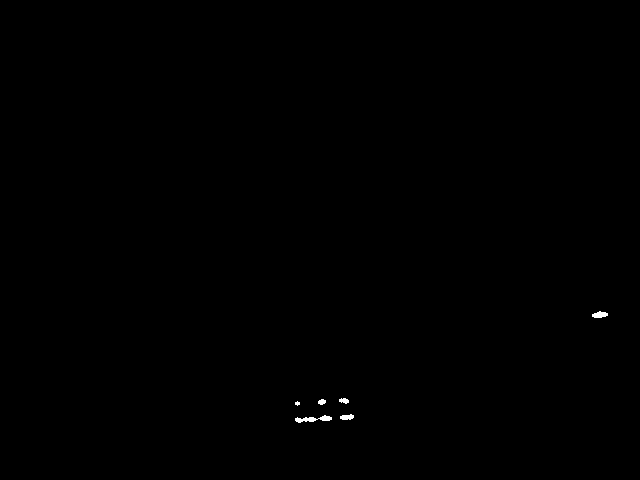
\includegraphics[width=0.2\textwidth]{ROS_gate3th2.png}}} \hspace{0.2 pt}
    \subfloat[ ]{\label{fig:ROS_gate3th3}{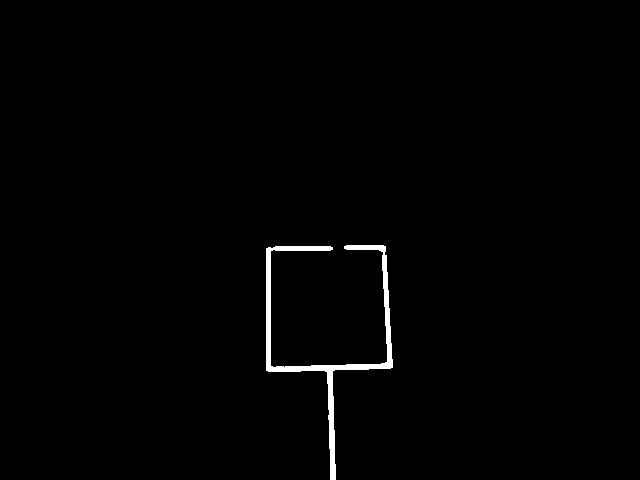
\includegraphics[width=0.2\textwidth]{ROS_gate3th3.png}}} \hspace{0.2 pt}
    \subfloat[ ]{\label{fig:ROS_gate3th4}{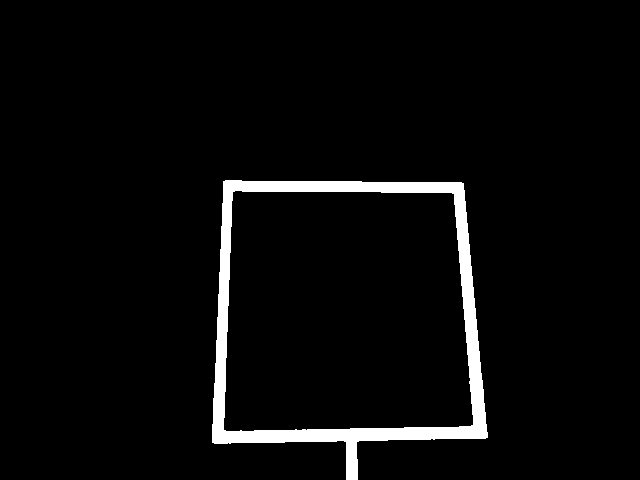
\includegraphics[width=0.2\textwidth]{ROS_gate3th4.png}}}
    
    \caption{Detección de la tercera compuerta}
    \label{fig:ROS_gate3}
\end{figure}

Por último, la figura \ref{fig:ROS_gate4} presenta la respectiva detección para la compuerta 4. En este caso se incluyen fotogramas en donde el dron se encuentra realizando un viraje durante la transición del waypoint. Al igual que en los otros casos, se aprecia que el dron requiere acortar la distancia para realizar el aislamiento por completo; sin embargo, a diferencia del caso anterior, en esta secuencia de fotogramas el dron sí fue capaz de detectar toda la estructura de la compuerta.

\begin{figure}[ht]
    \centering
    \subfloat[ ]{\label{fig:ROS_gate4og1}{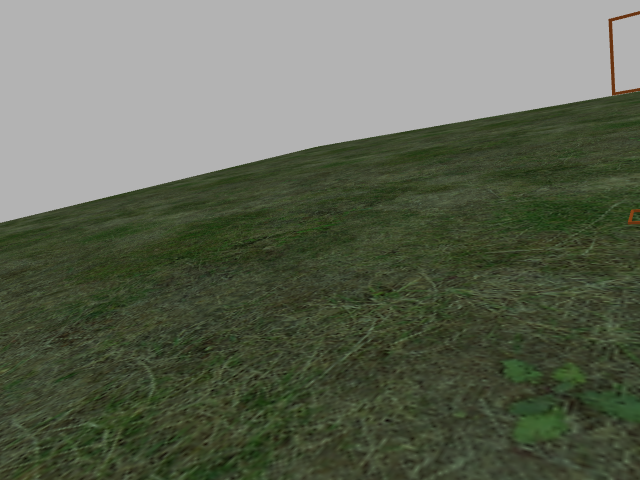
\includegraphics[width=0.2\textwidth]{ROS_gate4og1.png}}} \hspace{0.2 pt}
    \subfloat[ ]{\label{fig:ROS_gate4og2}{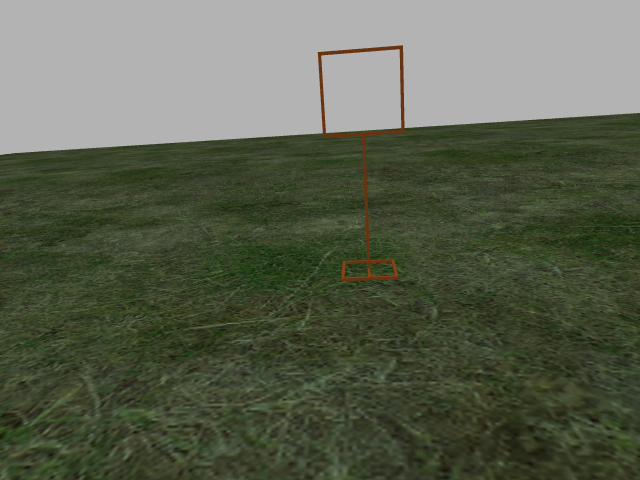
\includegraphics[width=0.2\textwidth]{ROS_gate4og2.png}}} \hspace{0.2 pt}
    \subfloat[ ]{\label{fig:ROS_gate4og3}{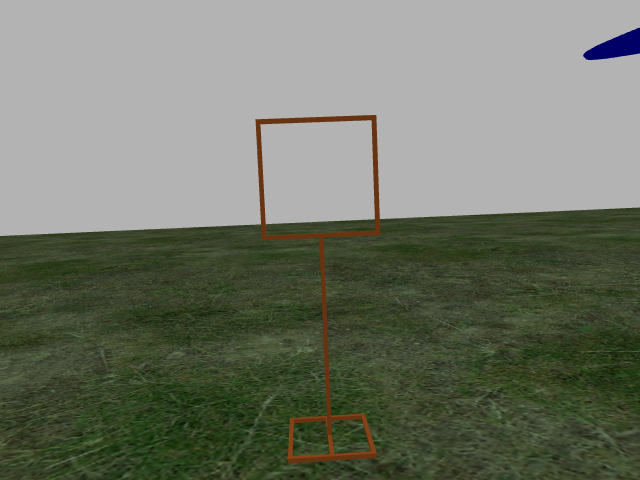
\includegraphics[width=0.2\textwidth]{ROS_gate4og3.png}}} \hspace{0.2 pt}
    \subfloat[ ]{\label{fig:ROS_gate4og4}{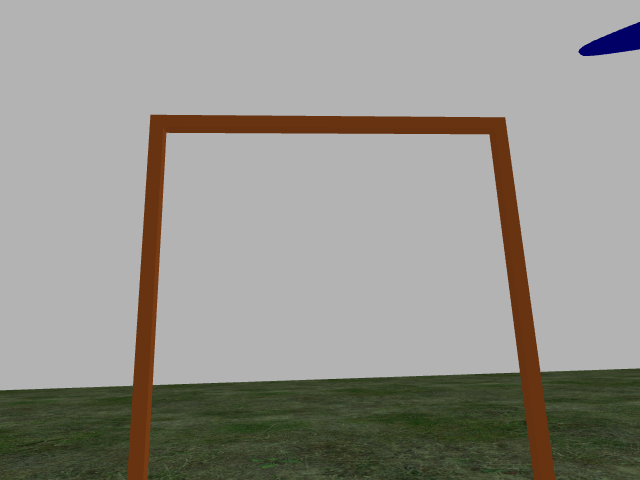
\includegraphics[width=0.2\textwidth]{ROS_gate4og4.png}}} \\
    \subfloat[ ]{\label{fig:ROS_gate4th1}{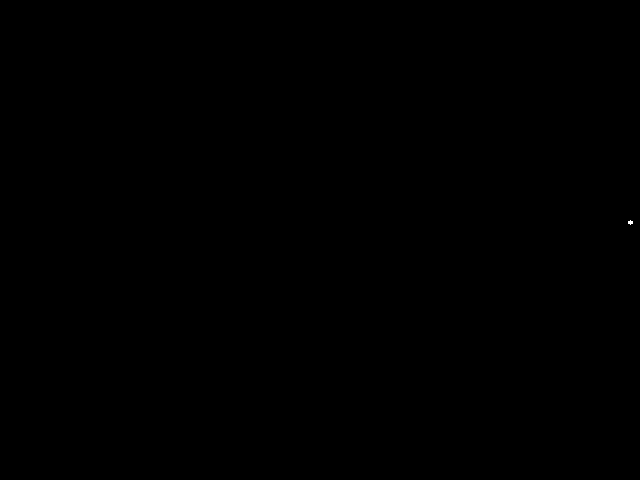
\includegraphics[width=0.2\textwidth]{ROS_gate4th1.png}}} \hspace{0.2 pt}
    \subfloat[ ]{\label{fig:ROS_gate4th2}{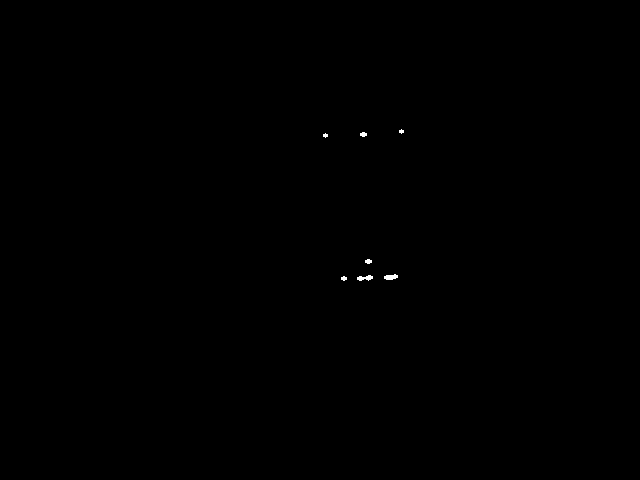
\includegraphics[width=0.2\textwidth]{ROS_gate4th2.png}}} \hspace{0.2 pt}
    \subfloat[ ]{\label{fig:ROS_gate4th3}{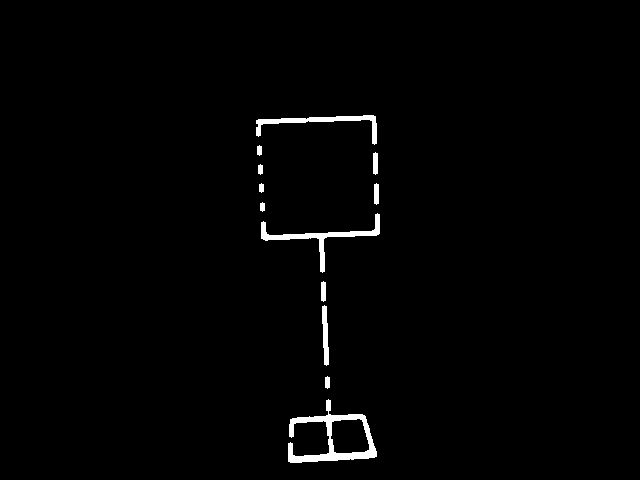
\includegraphics[width=0.2\textwidth]{ROS_gate4th3.png}}} \hspace{0.2 pt}
    \subfloat[ ]{\label{fig:ROS_gate4th4}{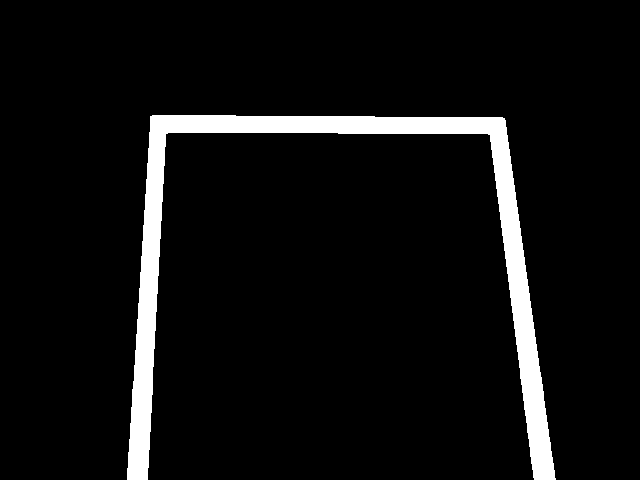
\includegraphics[width=0.2\textwidth]{ROS_gate4th4.png}}}
    
    \caption{Detección de la cuarta compuerta}
    \label{fig:ROS_gate4}
\end{figure}

A partir de los resultados observados, y a manera de síntesis, se puede decir que el algoritmo propuesto tiene un funcionamiento de cierta forma adecuado, pues logra detectar el objeto para el que fue sintonizado; sin embargo, el desempeño obtenido no fue el mejor, pues el dron necesita estar lo suficientemente cerca de la compuerta para realizar la detección, esto representa un comportamiento poco deseable, pues si en algún futuro se desea activar la transición de waypoints a partir de la detección de compuerta, no habría mucho tiempo de margen para maniobrar y dirigirse al siguiente waypoint. Además, con base en lo observado, el algoritmo no parece presentar la robustez necesaria para implementarlo en ambientes reales; sin embargo, esto último se encuentra fuera del alcance del presente trabajo y queda como propuesta para futuras implementaciones y análisis.


\section{Seguimiento de trayectoria}
A diferencia del algoritmo de visión artificial, la implementación del nodo para el seguimiento de trayectoria si representó un reto, principalmente por la problemática mencionada sobre la asincronía del firmware del piloto automático y la aplicación de seguimiento de trayectoria. Y es que la lógica seguida sigue siendo la misma, sin embargo, fue difícil encontrar una forma de crear un tiempo muerto o de espera, que permitiera que el piloto automático inicializara por completo, de tal manera que estuviera listo para recibir comando de vuelo y no anulara la ejecución de la secuencia de vuelo. 

Lo anterior representó un problema de gran relevancia pues el fin máximo de hacer el de los programas a nodos de ROS, fue el aprovechar la posibilidad de crear un lanzador que permitiera ejecutar todo el sistema utilizando un único comando y no 4 por separado. De tal forma que si la secuencia de vuelo es cancelada durante la ejecución del lanzador de procesos de ROS, se tendría que volver a ejecutar el programa de seguimiento de trayectoria de forma manual.

Lo anterior se pudo solventar implementando dos acciones en específico:

\begin{enumerate}
    \item Leer el estado del sistema y espera a que todos los sensores hayan sido inicializados
    \item Esperar el tiempo necesario para que el sistema arme los motores y se pueda proceder a la fase del despegue
\end{enumerate}

El primer punto se logró leyendo uno de los mensajes publicados por el piloto automático; \textit{SYS\_STATUS} entrega una serie de datos acerca del estado del sistema, entre ellos los estados de los sensores dentro de la simulación, de tal forma que la lectura de este parámetro devuelve un entero. A partir de las pruebas realizadas, se observó que cuando todos los sensores del sistema han sido inicializados el parámetro devuelve un valor de 1382128815, por lo que se implementó un ciclo que realizara la lectura del parámetro hasta que este tuviera el valor deseado. Una vez que los sensores han sido inicializados, se puede proceder con el resto de la secuencia de vuelo.

Ahora, previo al despegue es necesario indicarle al piloto automático que prepare los motores del dron para la secuencia del dron; sin embargo, esta acción conlleva un poco de tiempo, y si se envían comandos de vuelo de forma apresurada, el piloto automático rechaza las instrucciones, es por ello que se utilizó el método \textit{motors\_armed\_wait()} para pausar la secuencia de vuelo hasta que el sistema indique que los motores han sido armados de forma satisfactoria.

Con lo anterior se concluye la descripcción de la solución para los problemas enfrentados durante el porteo del Nodo de seguimiento de trayectoria. Ahora, la figura \ref{fig:pymav_flightmission} presenta una proyección en tres dimensiones de la trayectoria seguida por el dron tras la implementación del algoritmo de misión de vuelo. Realmente no se presenta ningún tipo de novedad, pues con base en la figura, se puede observar que la trayectoria de vuelo fue ejecutada de forma satisfactoria y corresponde a la misma trayectoria definida en la sección destinada al desarrollo del algoritmo por medio de scripts.

\begin{figure}[ht]
    \centering
    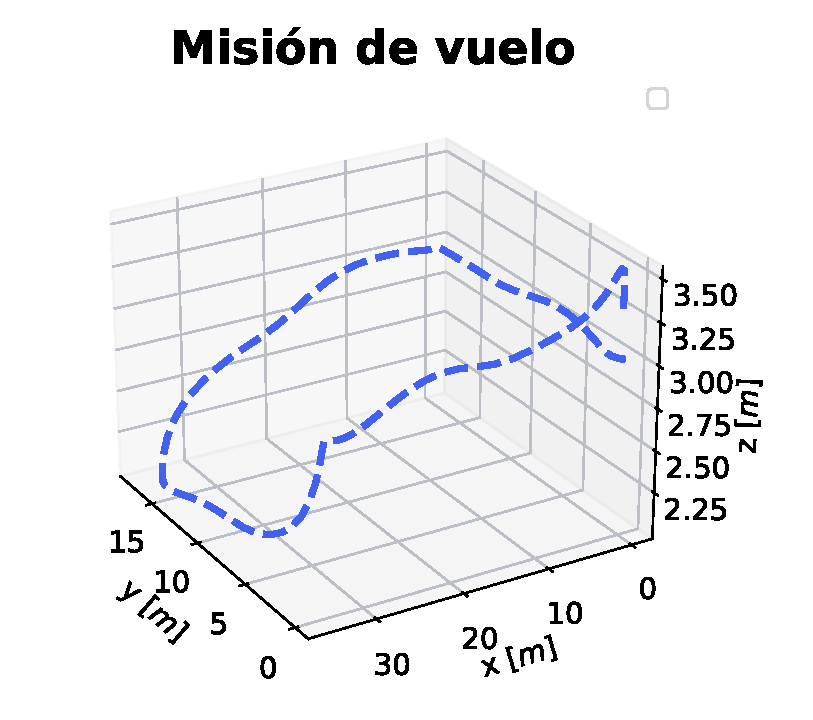
\includegraphics[width=0.45\textwidth]{pymav_flightmission.pdf}
    \caption{Recorrido realizado por el dron}
    \label{fig:pymav_flightmission}
\end{figure}

Adicionalmente, retomando las figuras \ref{fig:ROS_gate1og1}, \ref{fig:ROS_gate1og2}, \ref{fig:ROS_gate1og3} y \ref{fig:ROS_gate1og4} es posible observar parte de la trayectoria de vuelo desde la perspectiva de la cámara del dron. Por lo que, se puede decir con certeza que el seguimiento de trayectoria se implementó de manera correcta, logrando que el dron atravesara las 4 compuertas y completando el circuito de forma cíclica.

\section{Integración}
Por último, la integración del ambiente no solo conllevó el conjuntar los nodos creados en las secciones anterior, sino que, también se buscó la forma de implementar el SIL de Ardupilot y la simulación de Gazebo a partir de un archivo de lanzamiento en ROS. 

Dicho esto, el repositorio del proyecto cuenta con los archivos desarrollados para cada una de las etapas descritas en el capítulo de resultados; es decir, cuenta con todo lo necesario para recrear los resultados reportados en el presente documento y para utilizar el trabajo desarrollado, basta con clonar el repositorio y seguir las instrucciones de configuración del sistema descritas al inicio del capítulo.

A partir de todo lo que se ha discutido en esta sección, la figura \ref{fig:ROS_graph} muestra el diagrama de nodos que se genera al momento realizar el lanzamiento del sistema con ROS. Se puede observar que, en su conjunto, se desarrolló un sistema sencillo con dos nodos; el nodo designado como \textit{waypoints\_node} es el nodo encargado de ejecutar la secuencia de vuelo, mientras que el \textit{computer\_vision\_node} corresponde al nodo en donde se implementa el algoritmo de detección de compuerta. Adicionalmente, es posible observar otro nodo designado con el nombre de \textit{camera\_controller}, el cual es creado por el plugin que se encarga de entablar la comunicación entre ROS y Gazebo, de hecho, se puede observar el topic por donde se envían los fotogramas generados por la simulación hacia el nodo de visión artificial, el cual está designado como \textit{cam\_image\_raw}.

\begin{figure}[ht]
    \centering
    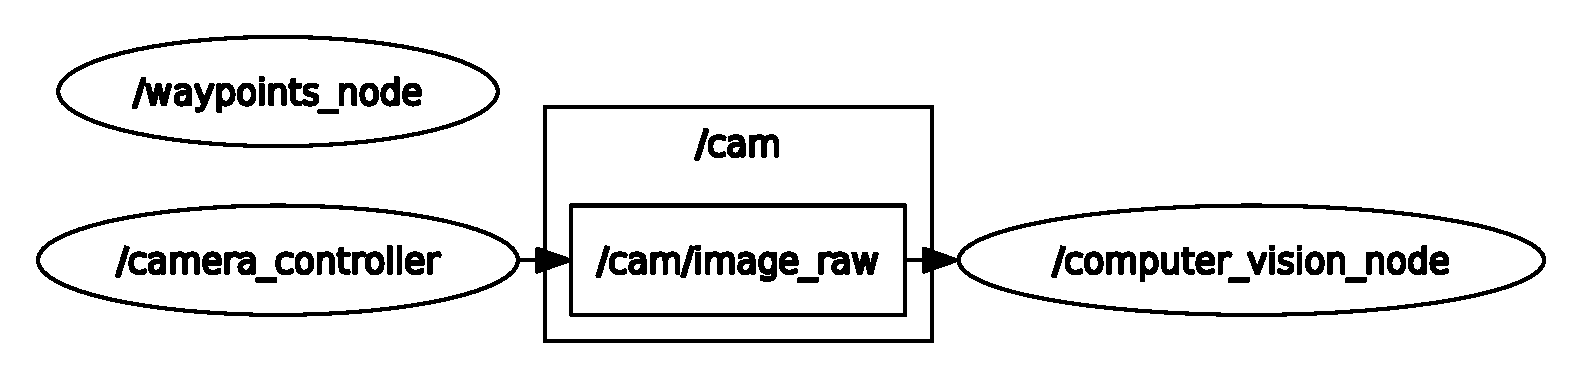
\includegraphics[width=0.7\textwidth]{ROS_graph.pdf}
    \caption{Recorrido realizado por el dron}
    \label{fig:ROS_graph}
\end{figure}


Además, cabe mencionar que a pesar de consultar distintas fuentes, la implementación de la ejecución del ambiente de simulación de Gazebo con un archivo de lanzamiento de ROS no fue posible, pues cuando la simulación se ejecuta de esta forma, no se genera de forma adecuada el ambiente; sin embargo, no existió ningún problema al momento de implementar el SIL de Ardupilot en el lanzador.

Por último, si el usuario siguió las instrucciones de configuración de forma adecuada y cuenta con los archivos del repositorio asociado a este trabajo, debería de ser capaz de ejecutar el sistema propuesto con dos simples comandos

\begin{lstlisting}[language = bash]
    $ ros2 launch adf_sil sil.launch.py
\end{lstlisting}

\begin{lstlisting}[language = bash]
    $ gazebo --verbose ../src/gazebo_sim/worlds/adr_circuit.world
\end{lstlisting}


El primero comando se encarga de ejecutar el nodo de visión artificial, misión de vuelo y el SIL de ArduPilot, mientras que el segundo inicializa el ambiente de simulación de Gazebo. El directorio especificado en este segundo comando puede variar dependiendo de donde se haya clonado el repositorio del proyecto.

A manera de recapitulación, se puede mencionar que se logró realizar el proteo de los algoritmos bases del sistema de vuelo a ROS, de tal forma que el algoritmo de visión artificial y el de seguimiento de trayectoria se ejecutaron como nodos de ROS, además, también fue posible implementar el framework de SIL de ArduPilot desde una archivo de lanzamiento de ROS. Por otro lado, no se pudo realizar la integración del ambiente de simulación dentro del archivo de lanzamiento, pues la simulación no se inicializaba de forma correcta al implementarla de esta manera; sin embargo, lo anterior no quiere decir que la integración final de los módulos de software haya fallado, sino que, de momento el ambiente de simulación tiene que ser ejecutado de forma individual para que interactúe de forma correcta con el resto de programas del sistema de vuelo.
A partir de todo lo ya mencionado en este capítulo, se da por concluido el apartado de resultados y se procede a concluir con base en todo lo observado a lo largo del trabajo.